\documentclass[useAMS,usenatbib]{mn2e}
\pdfoutput=1
\usepackage[varg]{txfonts}
\usepackage{astrojournals}
\usepackage{graphicx}
\usepackage{microtype}
\usepackage{xcolor}
\usepackage{fixltx2e}
\usepackage{hyperref}
\usepackage{siunitx}
\hypersetup{colorlinks=True, linkcolor=blue!50!black, citecolor=black,
  urlcolor=blue!50!black}

\usepackage[greek,english]{babel} 
\newcommand{\texttheta}{\greektext j\latintext}
\newcommand\thC{\texttheta\textsuperscript{1}\,Ori~C}

\begin{document}

%% Skip over the parts that are already written
\addtocounter{section}{6}
\addtocounter{subsection}{2}
\addtocounter{table}{5}
\addtocounter{figure}{9}


\begin{figure*}
  \centering
  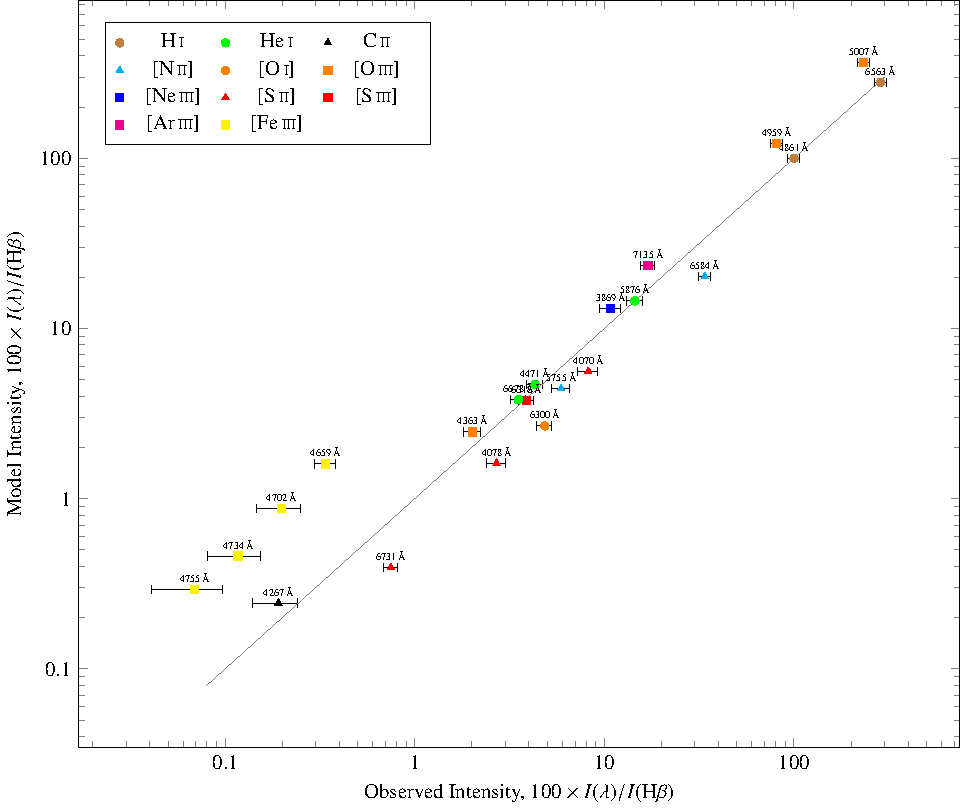
\includegraphics{ratios-figure-figure0}
  \caption{Comparison of model and observed line intensities for 177-341}
  \label{fig:model}
\end{figure*}

\subsection{A physical model of 177-341}
As an alternative to the purely empirical analysis presented in the previous sections, a different approach to analysing the emission spectrum of the proplyds is through the construction of physical models that combine a priori simulations of radiative transfer, hydrodynamics, and atomic physics in order to predict the density, temperature, and ionization structure of the proplyd flow.  
Such models have previously been applied to the ensemble properties of large numbers of proplyds \citep*{1998ApJ...499..758J, 1998AJ....116..322H} and in detail to individual objects such as 177-341 \citep{1999AJ....118.2350H}, LV2 \citep{2002ApJ...566..315H}, and LV1 \citep{2002ApJ...570..222G}. 
We have improved on these models in two significant ways.
First, whereas published models have considered only emission from regions where hydrogen is fully ionized and the flow is supersonic, we now use a detailed analytic model of gas acceleration in the ionization front \citep{2005ApJ...621..328H} to extend the treatment to cover partially ionized emission zones where the gas moves subsonically. 
Second, whereas published models used ad hoc fitting functions to the emissivity structure, specifically tailored to only the brightest emission lines, we now use the plasma micropysics code Cloudy \citep{1998PASP..110..761F} to self-consistently calculate the full physical structure and emission spectrum of the proplyd flow. 

\begin{table}
  \centering
  \caption{Input parameters for physical model of 177-341} 
  \begin{tabular}{ll}\hline
    Stellar spectrum:& 
    \(T_* = \SI{39000}{K}\)\\
    \citep{2006AandA...448..351S} & \(\log g = 4.1\)\\
    & \(L_* = \num{2.04e5}\,L_\odot\)\\
    Ionizing flux at proplyd:& 
    \(\Phi_{\mathrm{H}} = \SI{3.18e13}{cm^{-2} s^{-1}}\)
    \\
    Ionization front radius:& 
    \(r_0 = \SI{1.91e15}{cm}\)
    \\
    Gas-phase abundances: & Orion Nebula  \citep{2004MNRAS.355..229E}\\
    Dust composition: & Standard Orion \citep{1991ApJ...374..580B}\\
    \hline
  \end{tabular}
  \label{tab:model:pars}
\end{table}

Preliminary results of the emission line spectrum of such a model applied to 177-341 are shown in Figure~\ref{fig:model}.  
The input parameters for the model (values given in Table~\ref{tab:model:pars}) are the radius of the ionization front at the proplyd cusp (assumed hemispherical), the intensity and spectral shape of the illuminating stellar radiation, and the composition (gas-phase elemental mix and dust grain populations) of the proplyd material.  
For all these parameters, we simply took values from the literature, rather than trying to adjust them to fit the current observations.  
The stellar spectrum is that determined for \thC{} by spectroscopic analysis \citep{2006AandA...448..351S}. 
The ionization front radius is the value determined by fitting to \textit{HST} emission line images \citep{1999AJ....118.2350H}, while the separation of the proplyd from the ionizing star is taken to be 

    

The diffuse radiation field and the proplyd tail are ignored in this model, since the observational aperture (\S~2.2) only covers the proplyd head. 

\bibliographystyle{mn2e}
\bibliography{BibdeskLibrary}

\end{document}
